\chapter{Umsetzung}

\section{Gegebenheiten}

Die Umsetzung findet in einem Unternehmen mit weltweit rund 150 Standorten und 6700 Mitarbeitern (Stand Mai 2018) statt.
Es gibt eine zentrale Informatik mit einer eigenen Softwareentwicklungs-Abteilung, in der 4 Scrum-Teams angesiedelt sind.
Es wurde gezielt ein bestimmtes Scrum Team zur Umsetzung gewählt, weil dieses aus Sicht des Autors den Scrum Prozess bereits am weitesten entwicklet hat und dadurch Werkzeuge zur Prozessüberwachung dort am meisten Sinn machen.
Aus sicherheitstechnischen Gründen wird auf das Unternehmen in dieser Arbeit nicht weiter eingegangen.

\newpage
\section{Metriken Identifizieren}

\subsection{\ac{GQM}}

Um eine Vorauswahl an Metriken treffen zu können, wurden alle bisherigen Retrospektiven (es waren genau 15) analysiert und eine Topliste von Schlagwörtern der folgenden Fragestellungen aus den Retrospektiven erstellt:
\begin{enumerate}
    \item Welche guten Entscheidungen haben wir getroffen?
    \item Was haben wir gelernt?
    \item Was können wir besser machen?
    \item Was nervt uns noch immer?
\end{enumerate}

Dazu wurden die Ergebnisse in einer ElasticSearch Datenbank gespeichert und über eine sogenannte Terms Aggregation die wichtigsten Schlagwörter analysiert.
Bei der Indexierung werden die Wörter normalisiert, deshalb die teilweise andere Schreibweise (zum Beispiel wird aus Issue der Term issu).
Die Ergebnisse in Anhang~\ref{appendix:retros} sind für die einzelnen Punkte wie folgt interpretierbar:

\begin{description}
    \item[Welche guten Entscheidungen haben wir getroffen?] \hfill
    \begin{itemize}[noitemsep]
      \item Die ersten fünf Wörter lassen darauf schließen, dass das Team gut zusammenarbeitet, speziell bei der Wissensverteilung: Transparenz, Onboarding von neuen Themen und Pair-Programming.
      \item Ebenfalls lässt sich aus den weiteren Begriffen schließen, dass viel Wert auf Reviews, Daily und die Arbeitsweise an sich gelegt wird.
    \end{itemize}
    \item[Was haben wir gelernt?] \hfill
    \begin{itemize}[noitemsep]
      \item Auch hier spiegelt sich der Daten- und Kommunikationsfluss im Team wider.
      \item Die vielen Scrum Schlagwörter zeigen, dass die Retrospektiven richtig genutzt wurden, um den Prozess zu verbessern.
    \end{itemize}
    \item[Was können wir besser machen?] \hfill
    \begin{itemize}[noitemsep]
      \item Auch hier zeugen die Scrum Schlagwörter wieder von einer Prozessverbesserung und einem selbstreflektiven Verhalten.
      \item Die Dokumentation scheint teilweise noch ein Problem zu sein, diese kommt gleich zweimal vor.
      \item Issues scheinen teilweise nicht optimal zu sein. Da könnte das Schlagwort ``groß'' dazu passen.
      \item ``backlog'', ``blocked'' und ``àblauf'' lassen auf Probleme im Arbeitsablauf schließen.
    \end{itemize}
    \item[Was nervt uns noch immer?] \hfill
    \begin{itemize}[noitemsep]
      \item Hier lassen die Schlagwörter ``updat'', ``erreichbar'', ``infrastruktur'', ``jenkin'', ``test'' und ``umgebung'' auf ein Infrastruktur Problem schließen, welches das Team womöglich ausbremst.
      \item Die Schlagwörter ``lang'', ``groß'' und ``klar'' lassen auf Probleme mit Anforderungen beziehungsweise Stories schließen.
      \item ``apis'', ``dba'', ``laut'' und ``iso'' sind wahrscheinlich äußere Einflüsse, die bei der täglichen Arbeit stören.
    \end{itemize}
  \end{description}

Aus diesen Ergebnissen Lassen sich die \ac{GQM}-Modelle in Tabelle~\ref{tab:gqm-distraction},~\ref{tab:gqm-process} und~\ref{tab:gqm-issues} ableiten.

\begin{table}[H]
    \centering
    \begin{tabular}{llr}
    GOAL     & \begin{tabular}[c]{@{}l@{}}Absicht\\ Problem\\ Ressource\\ Sichtweise\end{tabular} & \begin{tabular}[c]{@{}l@{}}Verringerung\\ der Ablenkung\\ von Entwicklern\\ aus Sicht des Scrum Masters.\end{tabular} \\ \midrule
    QUESTION & \multicolumn{2}{l}{Wie viele Aufgaben erledigt das Team pro Sprint?} \\
    METRIC   & \multicolumn{2}{l}{Aufgaben-Volumen pro Sprint} \\ \midrule
    QUESTION & \multicolumn{2}{l}{Wie viele Aufgaben werden jeden Tag erledigt?} \\
    METRIC   & \multicolumn{2}{l}{\begin{tabular}[c]{@{}l@{}}erledigte Aufgaben pro Tag\\ Burn-down pro Tag\end{tabular}} \\ \midrule
    QUESTION & \multicolumn{2}{l}{Welche Tags haben als ``schlecht'' bewertete Aufgaben?} \\
    METRIC   & \multicolumn{2}{l}{\begin{tabular}[c]{@{}l@{}}Tags der Aufgaben, \\ um ``schlecht'' bewertete besser analysieren zu können\end{tabular}}
    \end{tabular}
    \caption{GQM\mbox{-}Modell \mbox{-} Ablenkung der Entwickler}\label{tab:gqm-distraction}
\end{table}

\begin{table}[H]
    \centering
    \begin{tabular}{llr}
    GOAL     & \begin{tabular}[c]{@{}l@{}}Absicht\\ Problem\\ Prozess\\ Sichtweise\end{tabular} & \begin{tabular}[c]{@{}l@{}}Optimierung\\ des Durchlaufes\\ im Entwicklungsprozess\\ aus Sicht des Scrum Teams.\end{tabular} \\ \midrule
    QUESTION & \multicolumn{2}{l}{Gibt es irgendwelche Engpässe im Prozess?} \\ 
    METRIC   & \multicolumn{2}{l}{Cumulative Flow} \\ \midrule
    QUESTION & \multicolumn{2}{l}{Wie lange dauert der Durchlauf einer Aufgabe?} \\
    METRIC   & \multicolumn{2}{l}{Lead Time}
    \end{tabular}
    \caption{GQM\mbox{-}Modell \mbox{-} Schwachstellen im Prozess}\label{tab:gqm-process}
\end{table}

\begin{table}[H]
    \centering
    \begin{tabular}{llr}
    GOAL     & \begin{tabular}[c]{@{}l@{}}Absicht\\ Problem\\ Ressource\\ Sichtweise\end{tabular} & \begin{tabular}[c]{@{}l@{}}Optimierung\\ der Aufgabengröße\\ im Backlog\\ aus Sicht des Product Owners.\end{tabular} \\ \midrule
    QUESTION & \multicolumn{2}{l}{Wie groß ist die Aufgabengröße im Durchschnitt?} \\
    METRIC   & \multicolumn{2}{l}{erledigte Story-Points / Aufgaben-Volumen} \\ \midrule
    QUESTION & \multicolumn{2}{l}{Wie lange dauert der Durchlauf einer Aufgabe?} \\
    METRIC   & \multicolumn{2}{l}{Lead-Time} \\ \midrule
    QUESTION & \multicolumn{2}{l}{Wie viele Aufgaben gehen im Entwicklungsprozess rückwärts?} \\
    METRIC   & \multicolumn{2}{l}{Aufgaben-Rückfälligkeit}
    \end{tabular}
    \caption{GQM\mbox{-}Modell \mbox{-} Aufgabengröße}\label{tab:gqm-issues}
\end{table}

\subsection{Umfrage im Team}

Zusätzlich zu der Analyse der Retrospektiven wurden dem Team Metriken und die Fragen, die damit beantwortet werden können, in Form einer Umfrage vorgestellt.
Die einzelnen Metriken wurden von den Teammitgliedern nach Wichtigkeit mit einer Skala von 1 bis 10 bewertet.
Anhang~\ref{appendix:questions} zeigt die Umfrage, wie sie den Teammitgliedern vorgelegt wurde und Anhang~\ref{appendix:answers} die dazugehörigen Antworten.
Die Ergebnisse wurden nach ihrem Druchschnittwert sortiert und die 10 als am wichtigsten bewerteten Metriken sind:

\begin{itemize}[noitemsep]
    \item \textbf{Burn Down (9,00)} \mbox{-} Erfüllt das Team seine Commitments? Plant das Team seine Arbeit realistisch?
    \item \textbf{Velocity (9,00)} \mbox{-} Wie konsistent arbeitet das Team?
    \item \textbf{Aufgaben-Volumen (8,57)} \mbox{-} Wie viel ungeplante Arbeit kam zum Sprint dazu? Wie groß ist die durchschnittliche Aufgabe? Gibt es Ausreißer?
    \item \textbf{Cumulative Flow (8,29)} \mbox{-} Gibt es Engpässe oder Schwachstellen im Prozess? Müssen gewisse Abläufe im Prozess optimiert werden?
    \item \textbf{Lead Time (8,14)} \mbox{-} Wie schnell können Aufgaben vom Team erledigt werden? Wie lange dauert die Umsetzung eines neuen Features?
    \item \textbf{Stresstests oder Benchmarking (7,86)} \mbox{-} Ist das Produkt auch noch unter Last verwendbar? Wie verändert sich die Leistung über die Zeit?
    \item \textbf{Code Coverage (7,71)} \mbox{-} Gibt es Module, die nicht oder schlecht getestet sind? Wie sieht die Entwicklung der Testabdeckung über die Zeit aus?
    \item \textbf{Bug Counts (7,57)} \mbox{-} Wie viele Fehler werden vom Team im Entwicklungsprozess übersehen? Wie viel ungeplante Arbeit kam zum Sprint dazu?
    \item \textbf{Aufgaben-Rückfälligkeit (7,57)} \mbox{-} Wie viele Aufgaben werden wieder in einen vorhergehenden Status gesetzt? Gibt es Probleme beim Verständnis der Aufgaben? Wie klar sind die Erwartungen des Teams an eine abgeschlossene Änderung (DoD)?
    \item \textbf{Bug-Erzeugungsrate (7,43)} \mbox{-} Wie viele Fehler wurden zu einem bestimmten Zeitpunkt erzeugt?
\end{itemize}

Außerdem wurde in den offenen Fragen am Ende zweimal gefordert, dass die Flüchtigkeit von Anforderungen Sichtbar wird. 
Dies kann zum einen durch die oben genannte Aufgaben-Rückfälligkeit und andererseits durch folgende Metrik abgebildet werden:

\begin{itemize}[noitemsep]
    \item \textbf{Anforderungen-Flüchtigkeit} \mbox{-} Wie oft wurde die Anforderung der Aufgabe angepasst?
\end{itemize}

\newpage
\section{Software}

Das für die Umsetzung gewählte Unternehmen setzt bereits auf Java als bevorzugte Programmiersprache und hat die in Kapitel~\ref{vorgehen:software} genannten Systeme im Einsatz.
Dadurch sind die Plattform und die zu unterstützenden Systeme vorgegeben.
Abbildung~\ref{fig:position_software} zeigt die Position in einer möglichen Systemlandschaft.

\begin{savenotes}
    \begin{figure}[H] 
        \centering
            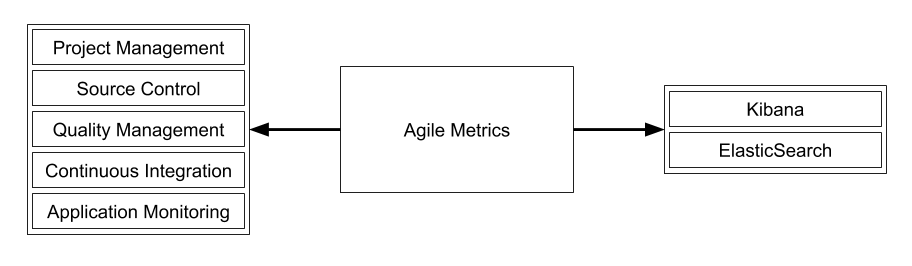
\includegraphics[width=0.8\textwidth]{img/position-overview.png}
        \caption{Position der Software}\label{fig:position_software}
    \end{figure}
\end{savenotes}

\subsection{Architektur}

Abbildung~\ref{fig:overview_architecture} zeigt das Architekturkonzept der Software (Agile Metrics).
Diese bildet eine Schnittstelle zwischen den einzelnen Systemen des Entwicklungsprozesses und dem System zur Darstellung der Metriken (in diesem Fall der sogenannte Elastic Stack~\footcite{elastic_stack} mit ElasticSearch und Kibana).
ElasticSearch ist dabei die Datenbank für die Metriken, genau genommen eine volltext-indizierte \ac{NoSQL}-Datenbank.
Kibana dient zur Darstellung der in der ElasticSearch-Datenbank gespeicherten Metriken.

\begin{savenotes}
    \begin{figure}[H] 
        \centering
            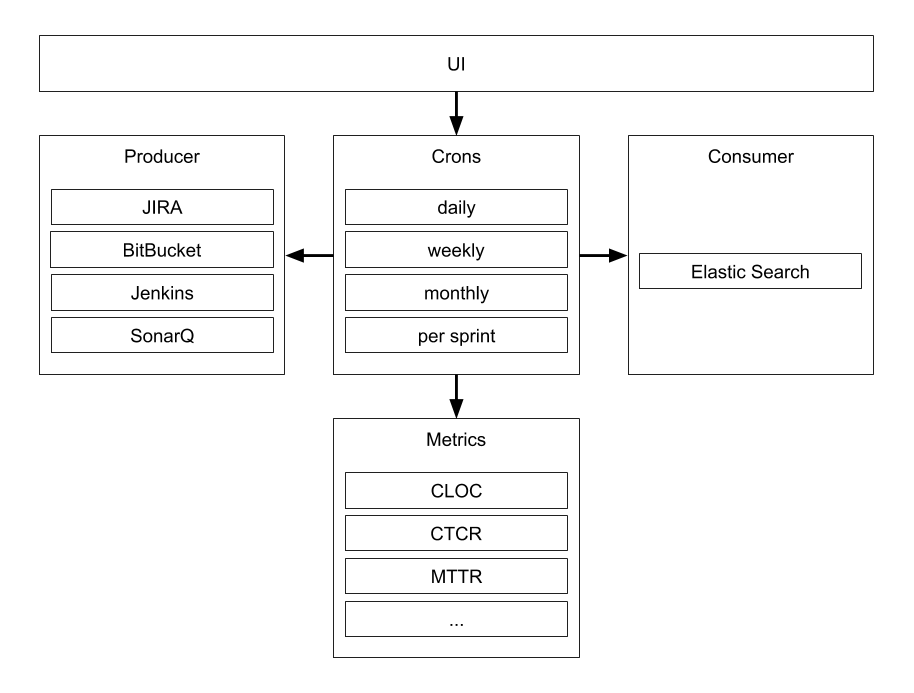
\includegraphics[width=0.8\textwidth]{img/architecture-overview.png}
        \caption{Übersicht der Software-Architektur}\label{fig:overview_architecture}
    \end{figure}
\end{savenotes}

\begin{description}
    \item[API] \hfill \\ Bietet eine RESTful Schnittstelle zum Abfragen des aktuellen Status.
    \item[Producer] \hfill \\ Sind Schnittstellen zu allen Systemen, die Messdaten erzeugen.
    \item[Cron] \hfill \\ Zeitsteuerung der Messdaten-Abfrage und Koordination der Erzeugung und Konsumierung von Metriken.
    \item[Metric] \hfill \\ Metriken, welche aus den Messdaten erzeugt und konsumiert werden.
    \item[Consumer] \hfill \\ Sind Schnittstellen zu allen Systemen, die Messdaten und Metriken konsumieren.
\end{description}

\subsection{Lizenz}

Bei der Recherche wurde keine Software gefunden, welche die oben genannten Funktionalitäten anbietet.
Daher wird die im Zuge dieser Arbeit erstellte Software quelloffen (OpenSource) angeboten.
Als Lizenz wurde dabei die MIT-Lizenz~\footcite{mit_license} gewählt, da sie eine einfache und großzügige Lizenz ist, die lediglich die Erhaltung des Urheberrechts und eine Lizenzangabe erfordert.

\subsection{\ac{VCS}, \ac{CI} und \ac{QS}}

Da es sich um eine quelloffene Software handelt, wird als \ac{VCS} ein öffentliches Repository~\footcite{agile_metrics_repo} in GitHub verwendet.
In diesem sind der Quellcode und die Veröffentlichungen der Software zugänglich.
Zusätzlich wird über GitHub Pages eine statische Seite~\footcite{agile_metrics_page} für das Projekt bereitgestellt, wie in Abbildung~\ref{fig:github_pages} ersichtlich.

\begin{savenotes}
    \begin{figure}[H] 
        \centering
            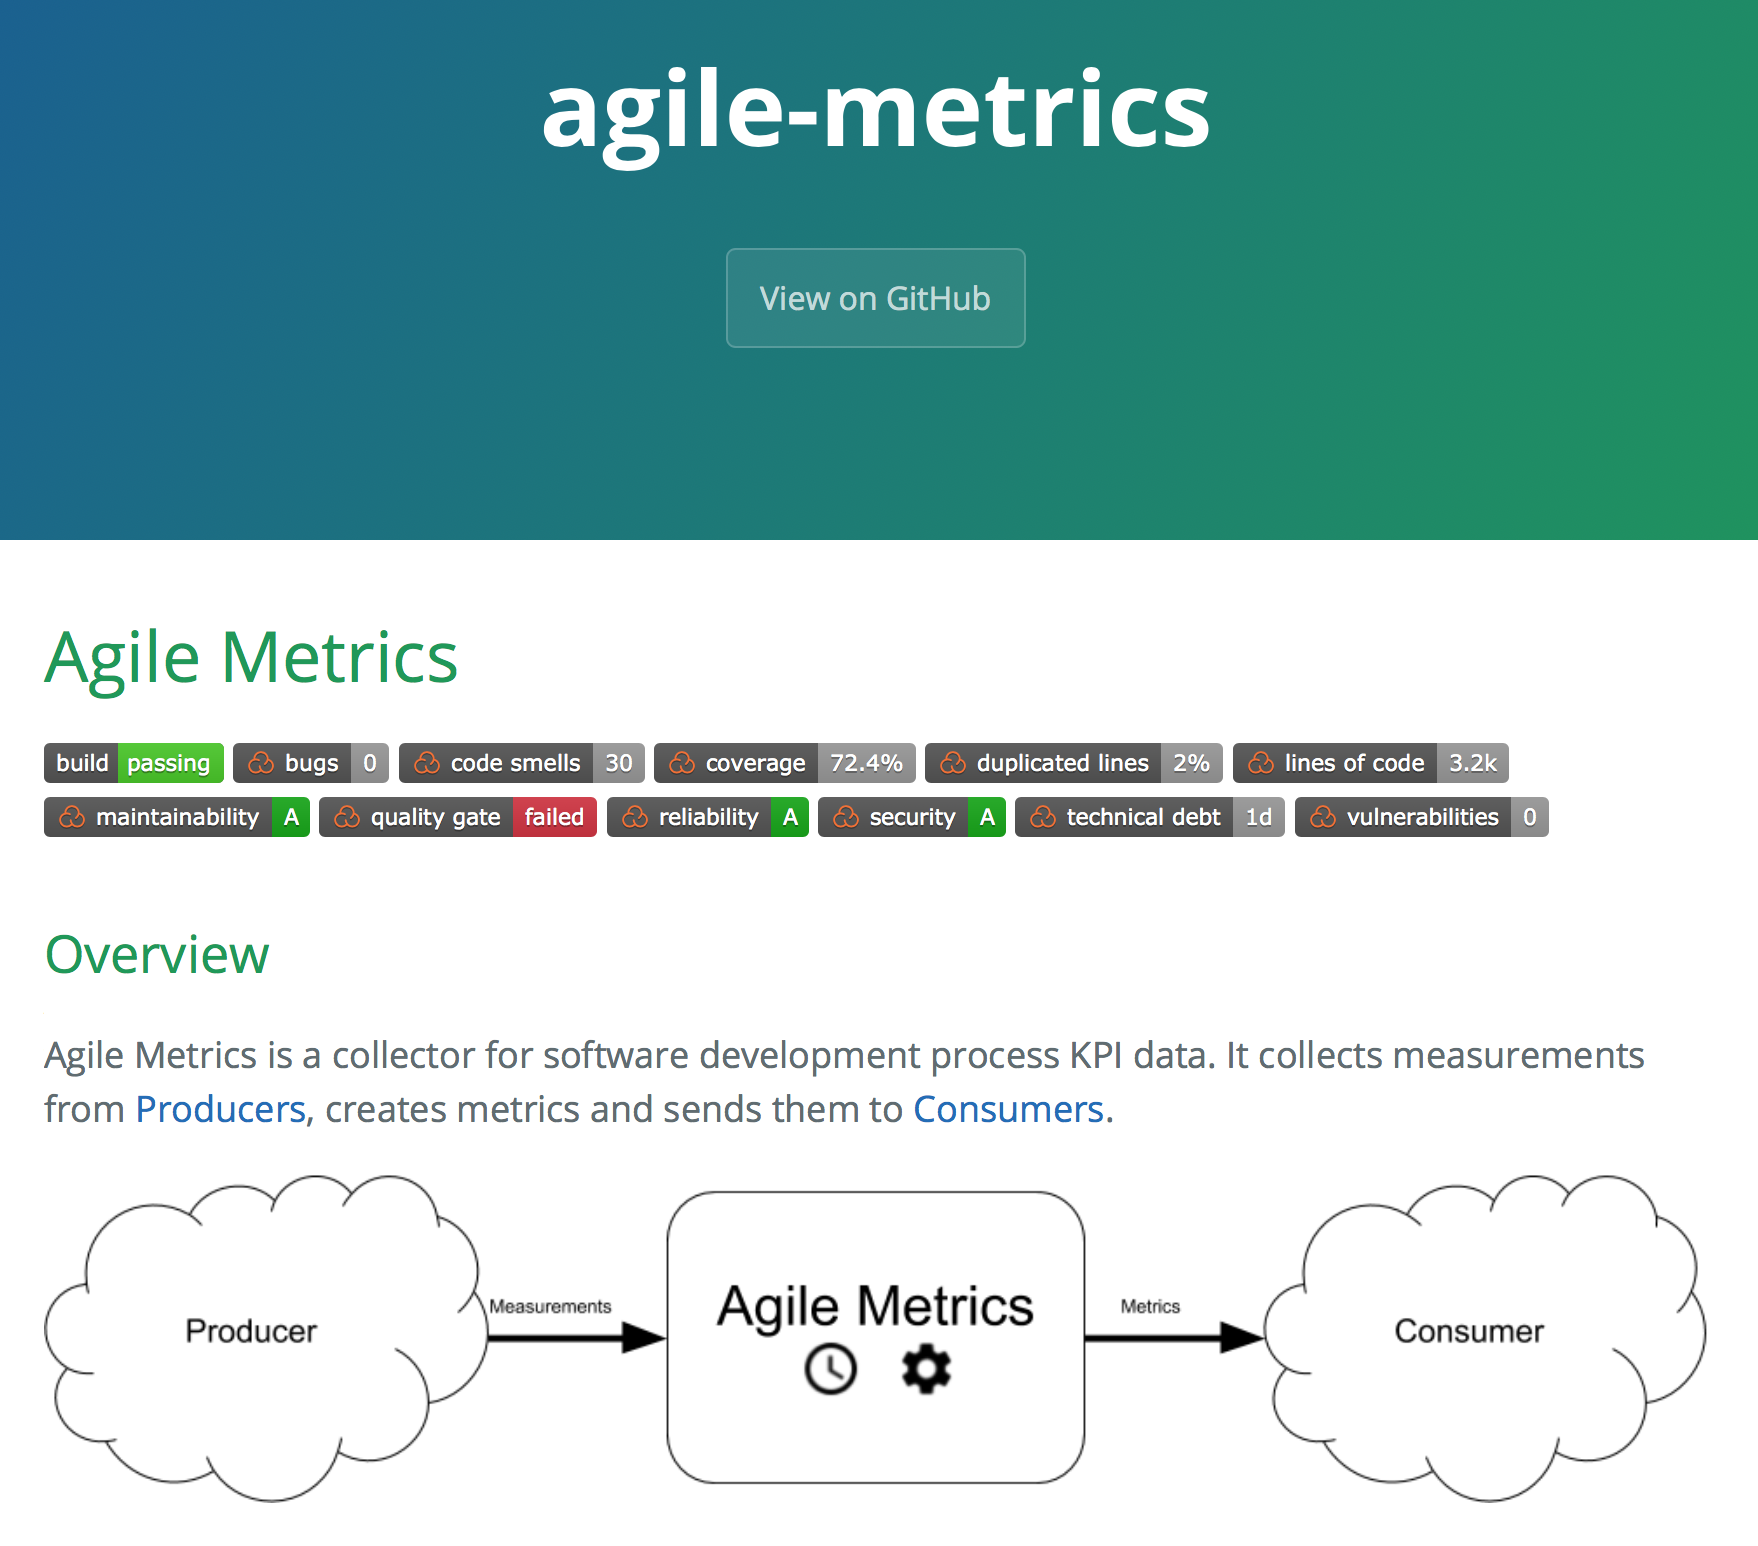
\includegraphics[width=0.8\textwidth]{img/github-pages.png}
        \caption{GitHub Pages - Agile Metrics}\label{fig:github_pages}
    \end{figure}
\end{savenotes}

Travis CI~\footcite{travis_agile_metrics} bietet einen kostenlosen \ac{CI}-Service und SonarCloud~\footcite{sonarcloud_agile_metrics} einen kostenlosen \ac{QS}-Service für quelloffene Projekte.

\begin{savenotes}
    \begin{figure}[H] 
        \centering
            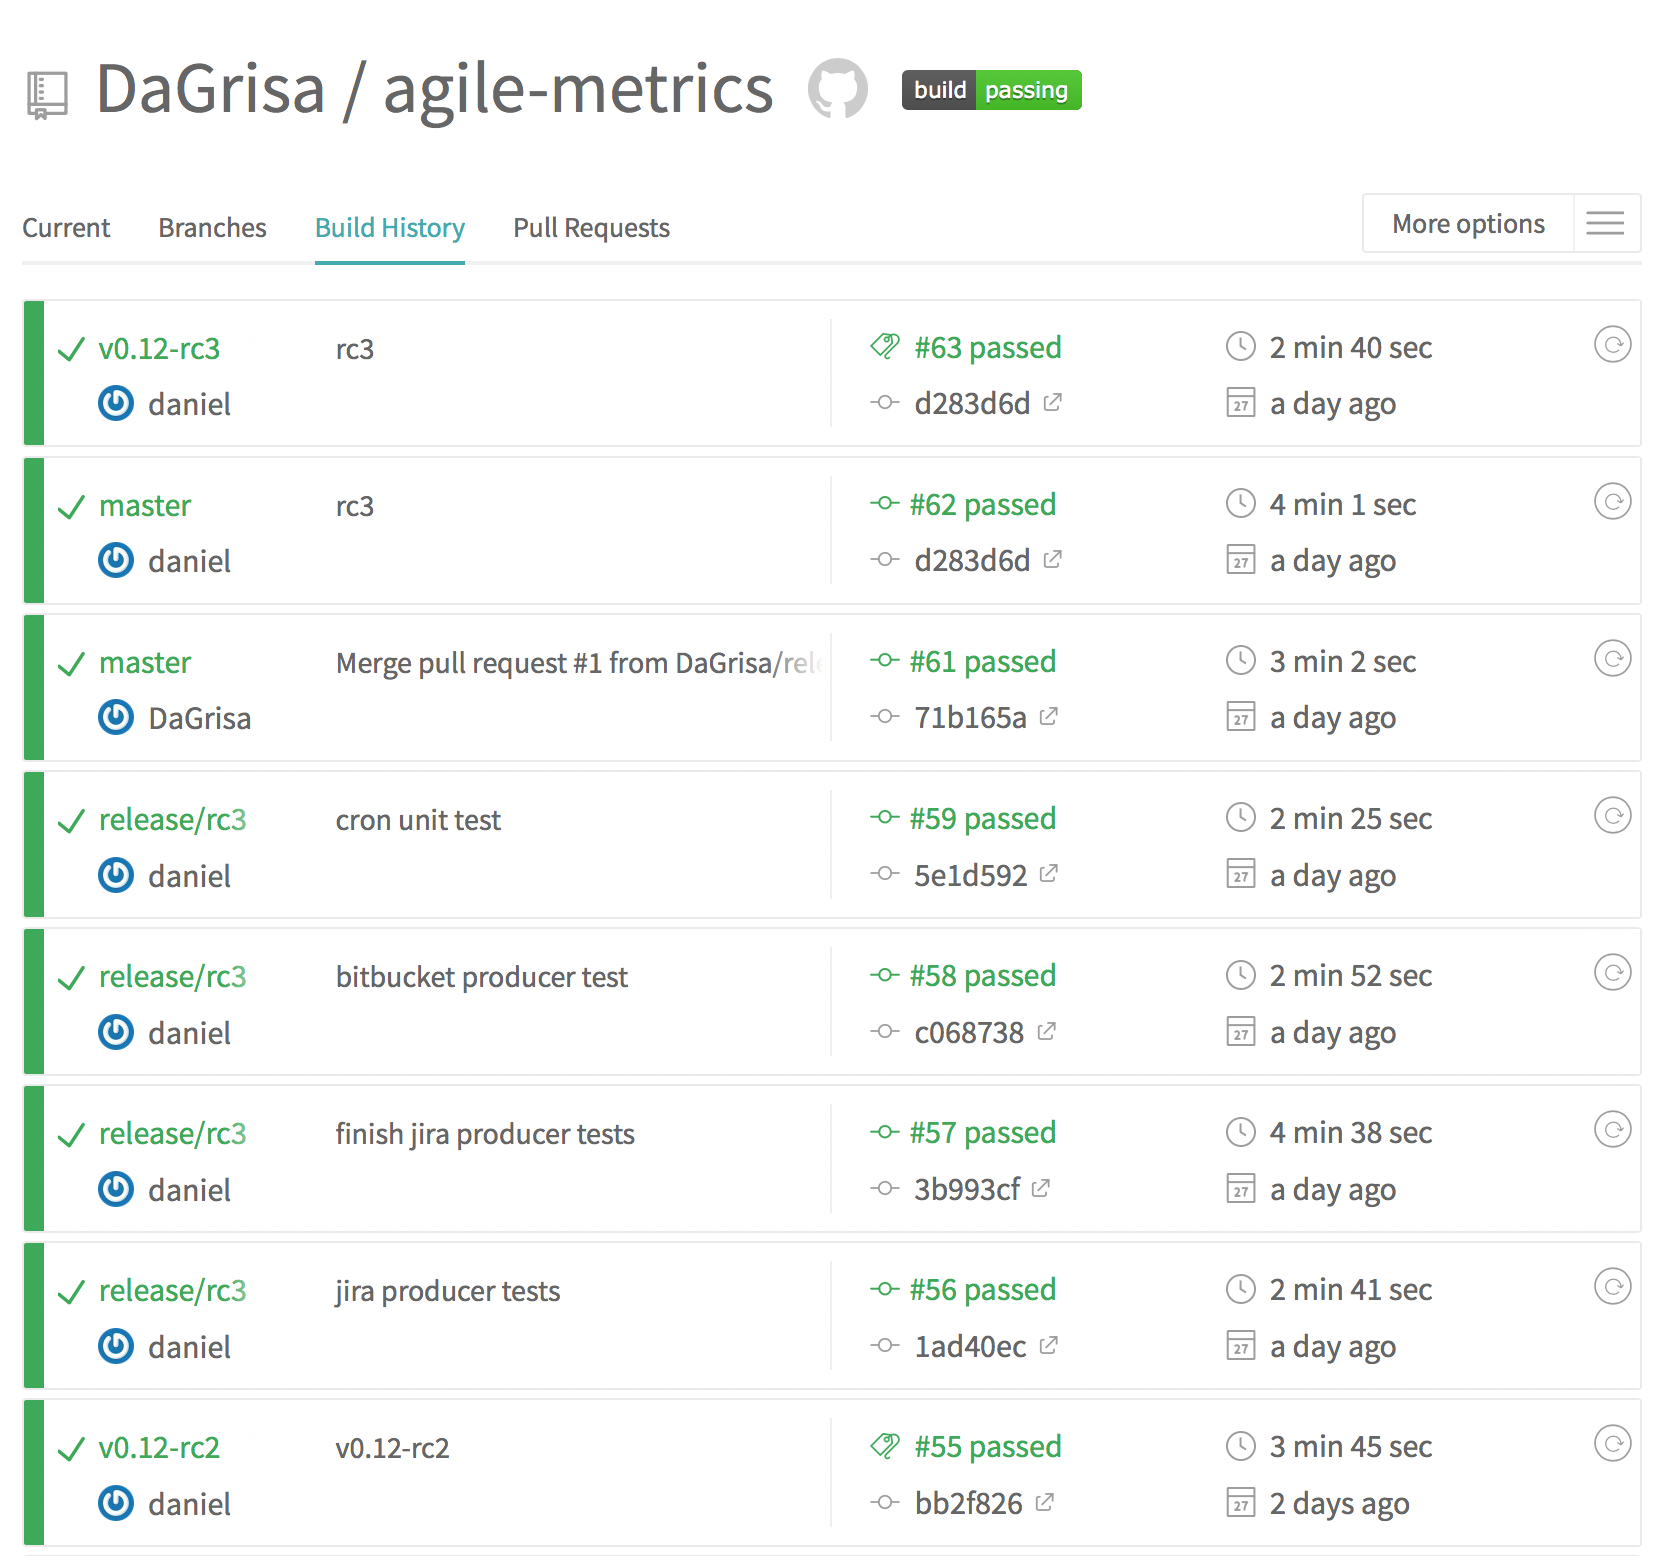
\includegraphics[width=0.8\textwidth]{img/travisci.png}
        \caption{Travis CI - Agile Metrics}\label{fig:travisci}
    \end{figure}
\end{savenotes}

Nach jedem Commit in das GitHub Repository wird ein Build gestartet, um kontinuierliche Integration zu gewährleisten.
Abbildung~\ref{fig:travisci} zeigt die Liste der zu diesem Zeitpunkt zuletzt durchgeführten Builds mit einigen Informationen.

\begin{savenotes}
    \begin{figure}[H] 
        \centering
            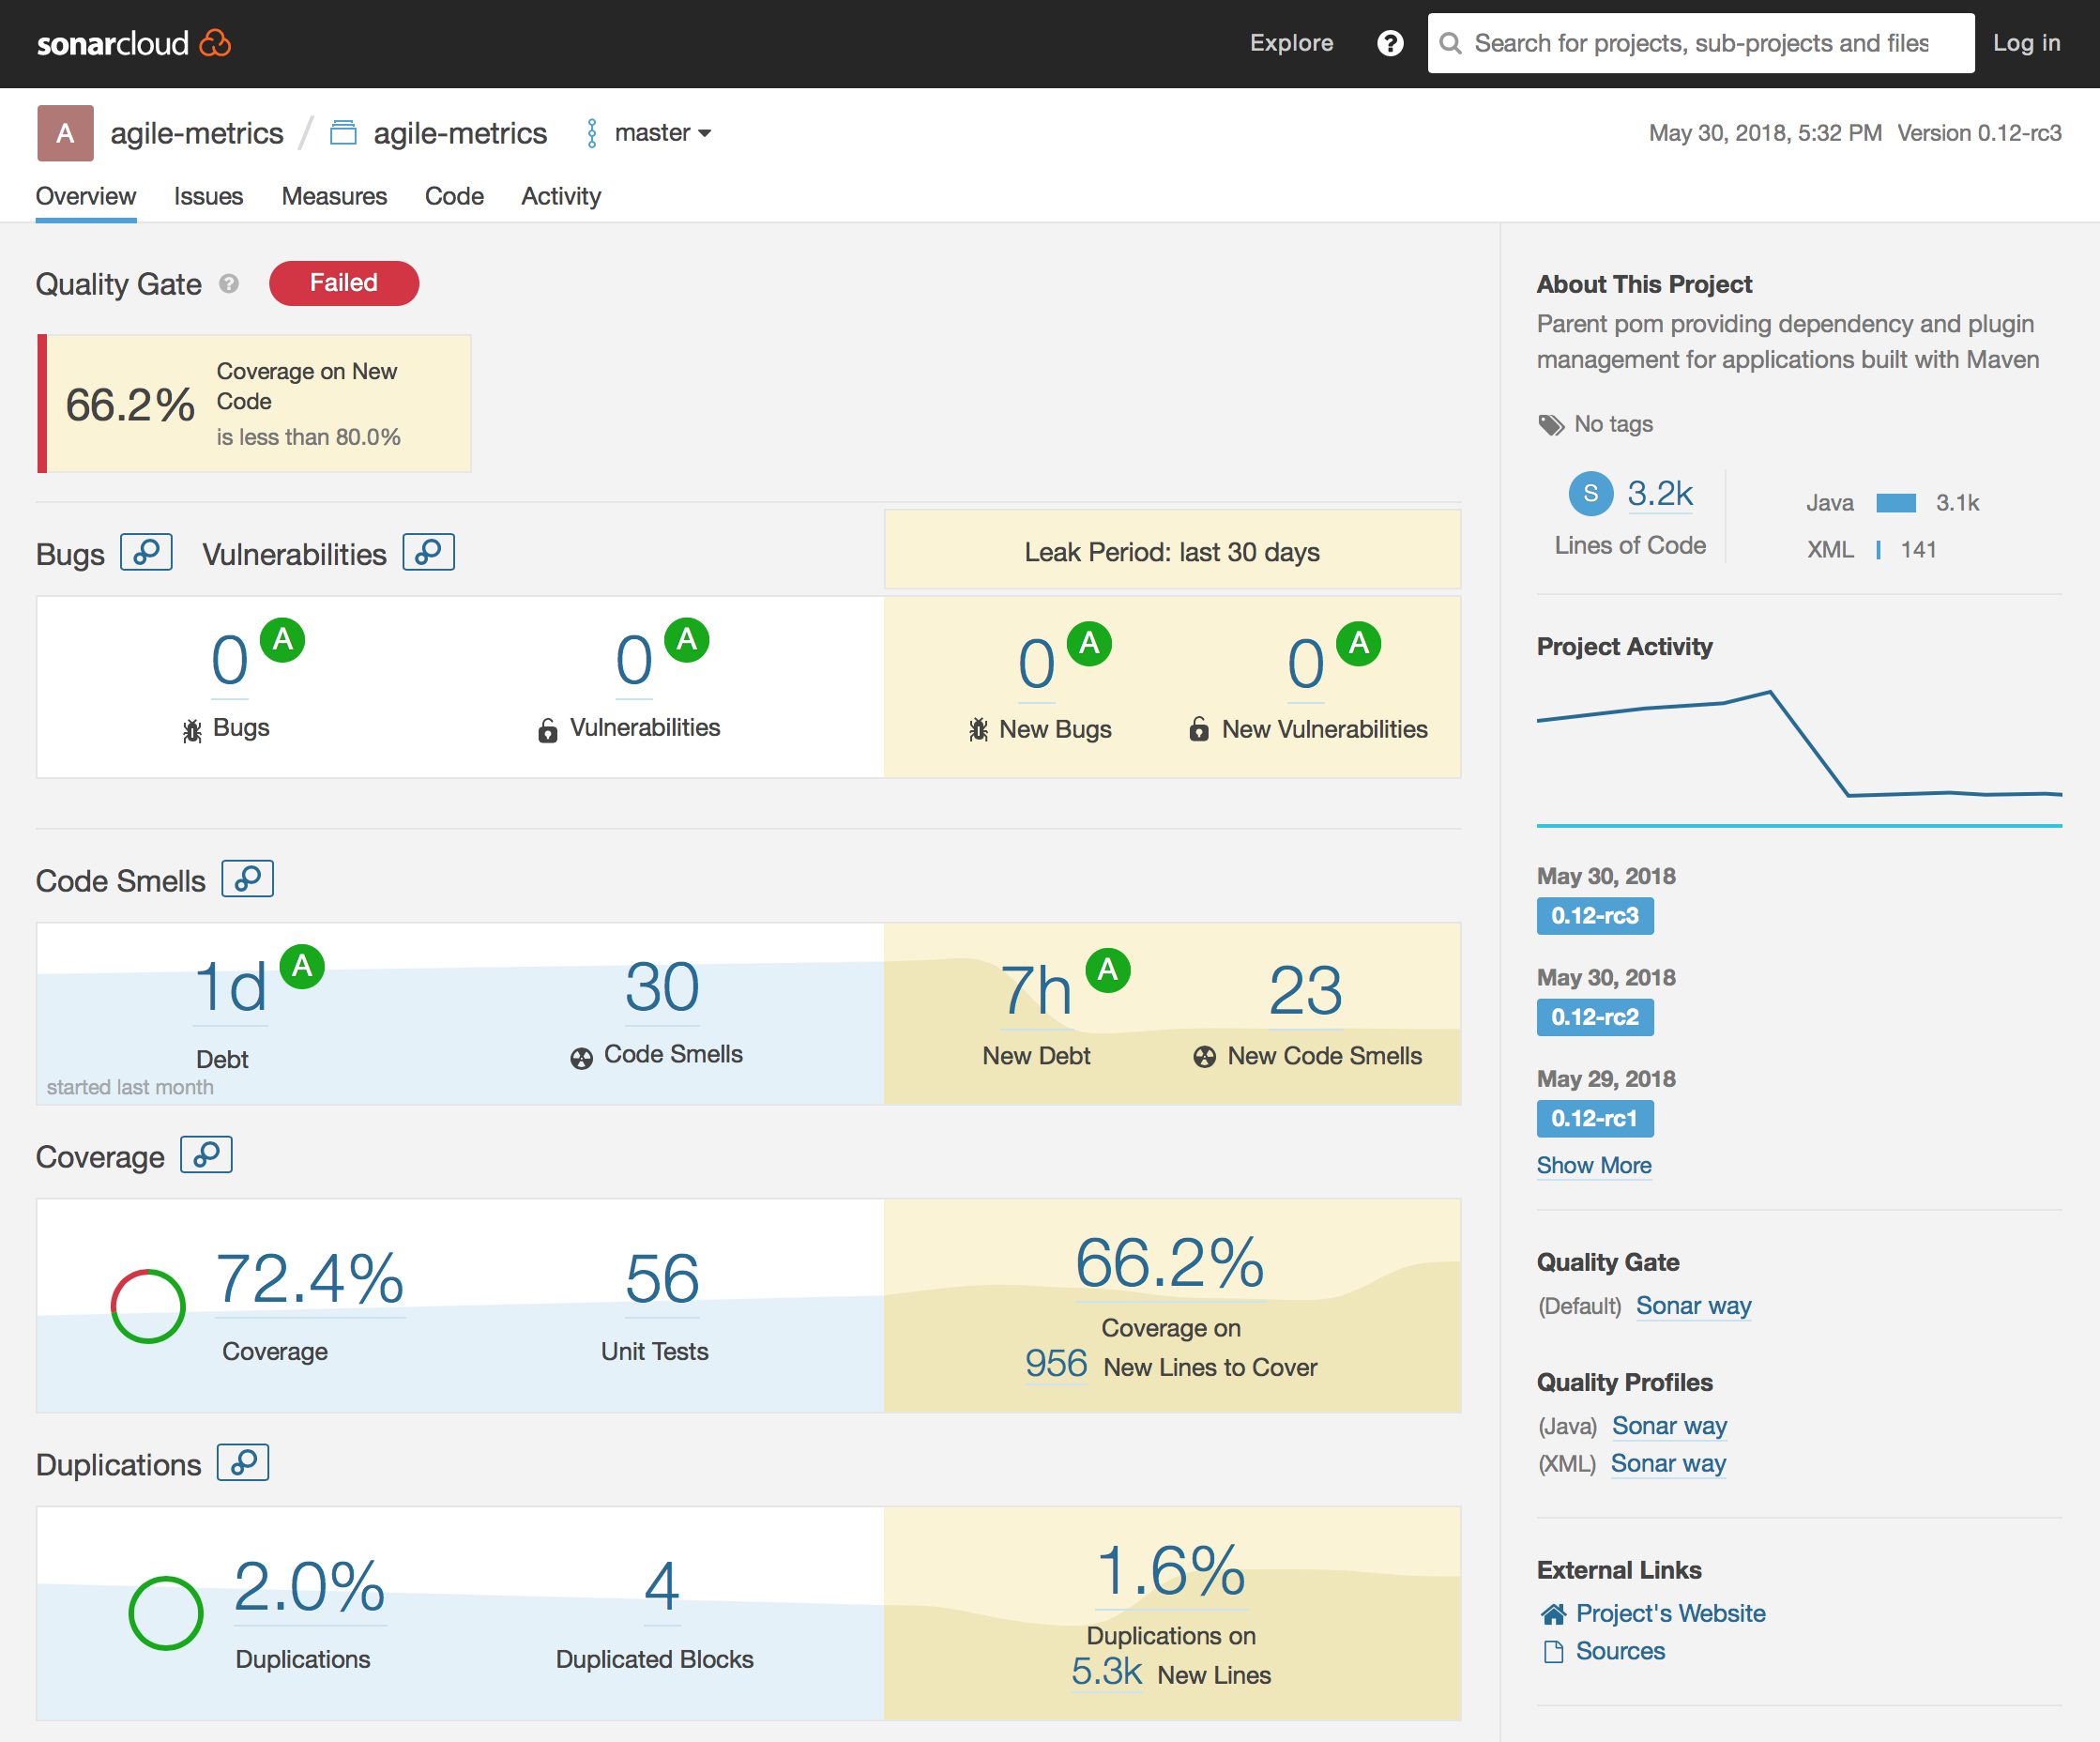
\includegraphics[width=0.8\textwidth]{img/sonarcloud.png}
        \caption{SonarCloud - Agile Metrics}\label{fig:sonarcloud}
    \end{figure}
\end{savenotes}

Jeder Build in Travis CI sendet mit Hilfe eines Addons Informationen über die Qualität des Quellcodes an SonarCloud.
Abbildung~\ref{fig:sonarcloud} zeigt die Übersichtsseite von SonarCloud mit den wichtigsten Qualitätsmetriken für das Projekt.

\newpage
\section{Inbetriebnahme}

Betrieben wird die Software auf einem eigens für Java Applikationen bereitgestellten Server. 
Wichtig dabei ist, dass alle benötigten Systeme erreichbar sind. 
Es wird auch ein Webproxy unterstützt, dieser kann in den Einstellungen konfiguriert werden.
Folgende Schritte sind notwendig, um Agile-Metrics in Betrieb zu nehmen:
\begin{description}
    \item[Neuestes Release] aus dem Repository auf GitHub herunterladen (zu diesem Zeitpunkt aktuellster Stand ist v1.0) und im gewünschten Verzeichnis ablegen, in dem es später laufen soll.
    \item[Einstellungen] in der Konfigurationsdatei (application.properties) vornehmen, wie in der Beschreibung der Software (README.md) näher erklärt. Benötigt werden hier vor allem die Zugangsdaten zu den einzelnen Systemen und einige Einstellungen für die Systeme selbst.
    \item[Service] einrichten, wenn benötigt. Das unterscheidet sich je nach Betriebssystem und muss dafür individuell recherchiert werden.
    \item[Logdatei] auf etwaige Fehler oder Probleme überprüfen (/logs/rollingfile.log). Beim Start werden die Zugangsdaten der Systeme gestestet und das Ergebnis in die Logdatei geschrieben, wie in Abbildung~\ref{fig:successful-start} ersichtlich.
\end{description}

\begin{savenotes}
    \begin{figure}[H] 
        \centering
            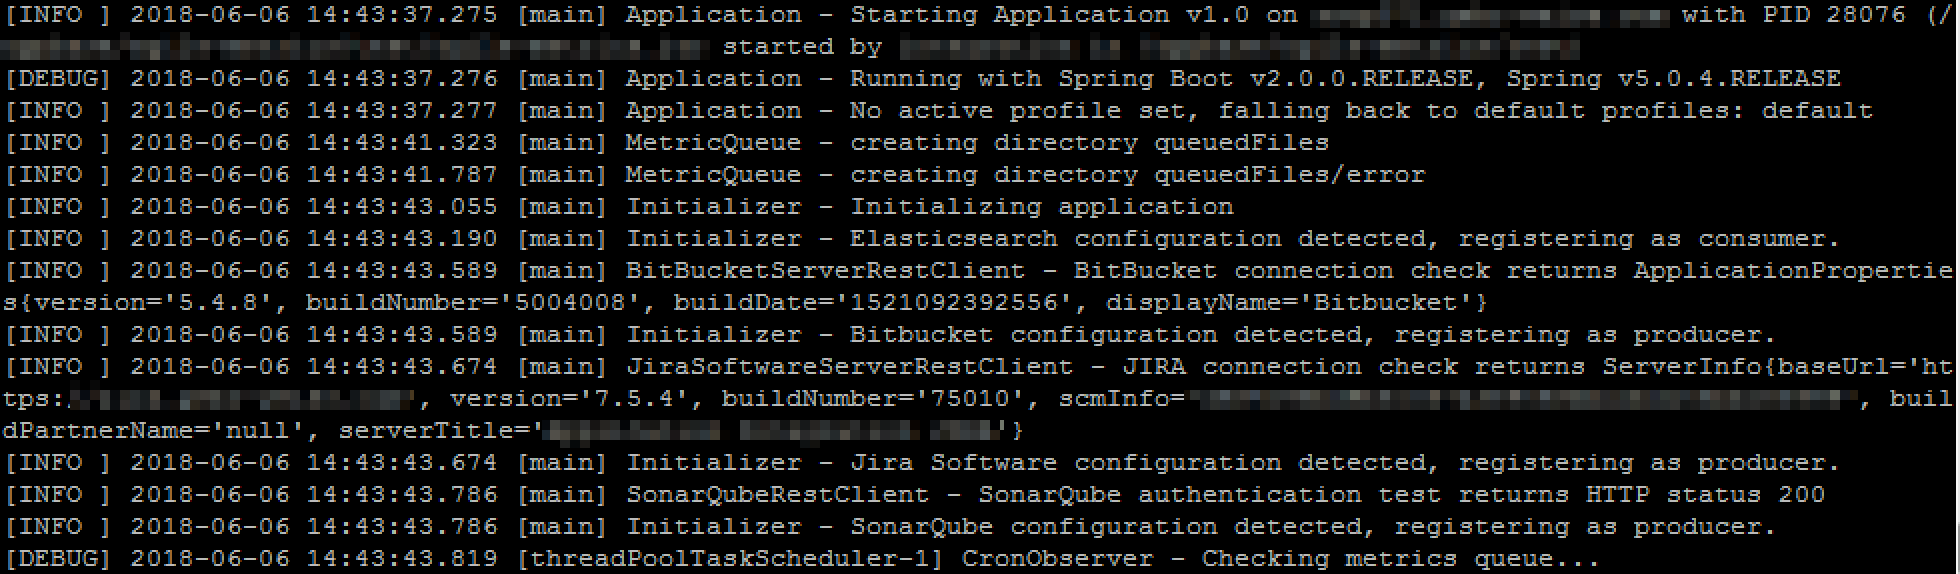
\includegraphics[width=1.0\textwidth]{img/successful-start.png}
        \caption{Logausgaben bei erfolgreichem Start}\label{fig:successful-start}
    \end{figure}
\end{savenotes}

Wird die Uhrzeit für den täglichen Durchlauf nicht anders eingestellt, werden ab dann täglich alle Metriken um 00:15 generiert und abgelegt.
Diese Metriken können dann visualisiert werden, wie in diesem Fall in Kibana.

\subsection{Visualisierte Ergebnisse}

\begin{savenotes}
    \begin{figure}[H] 
        \centering
            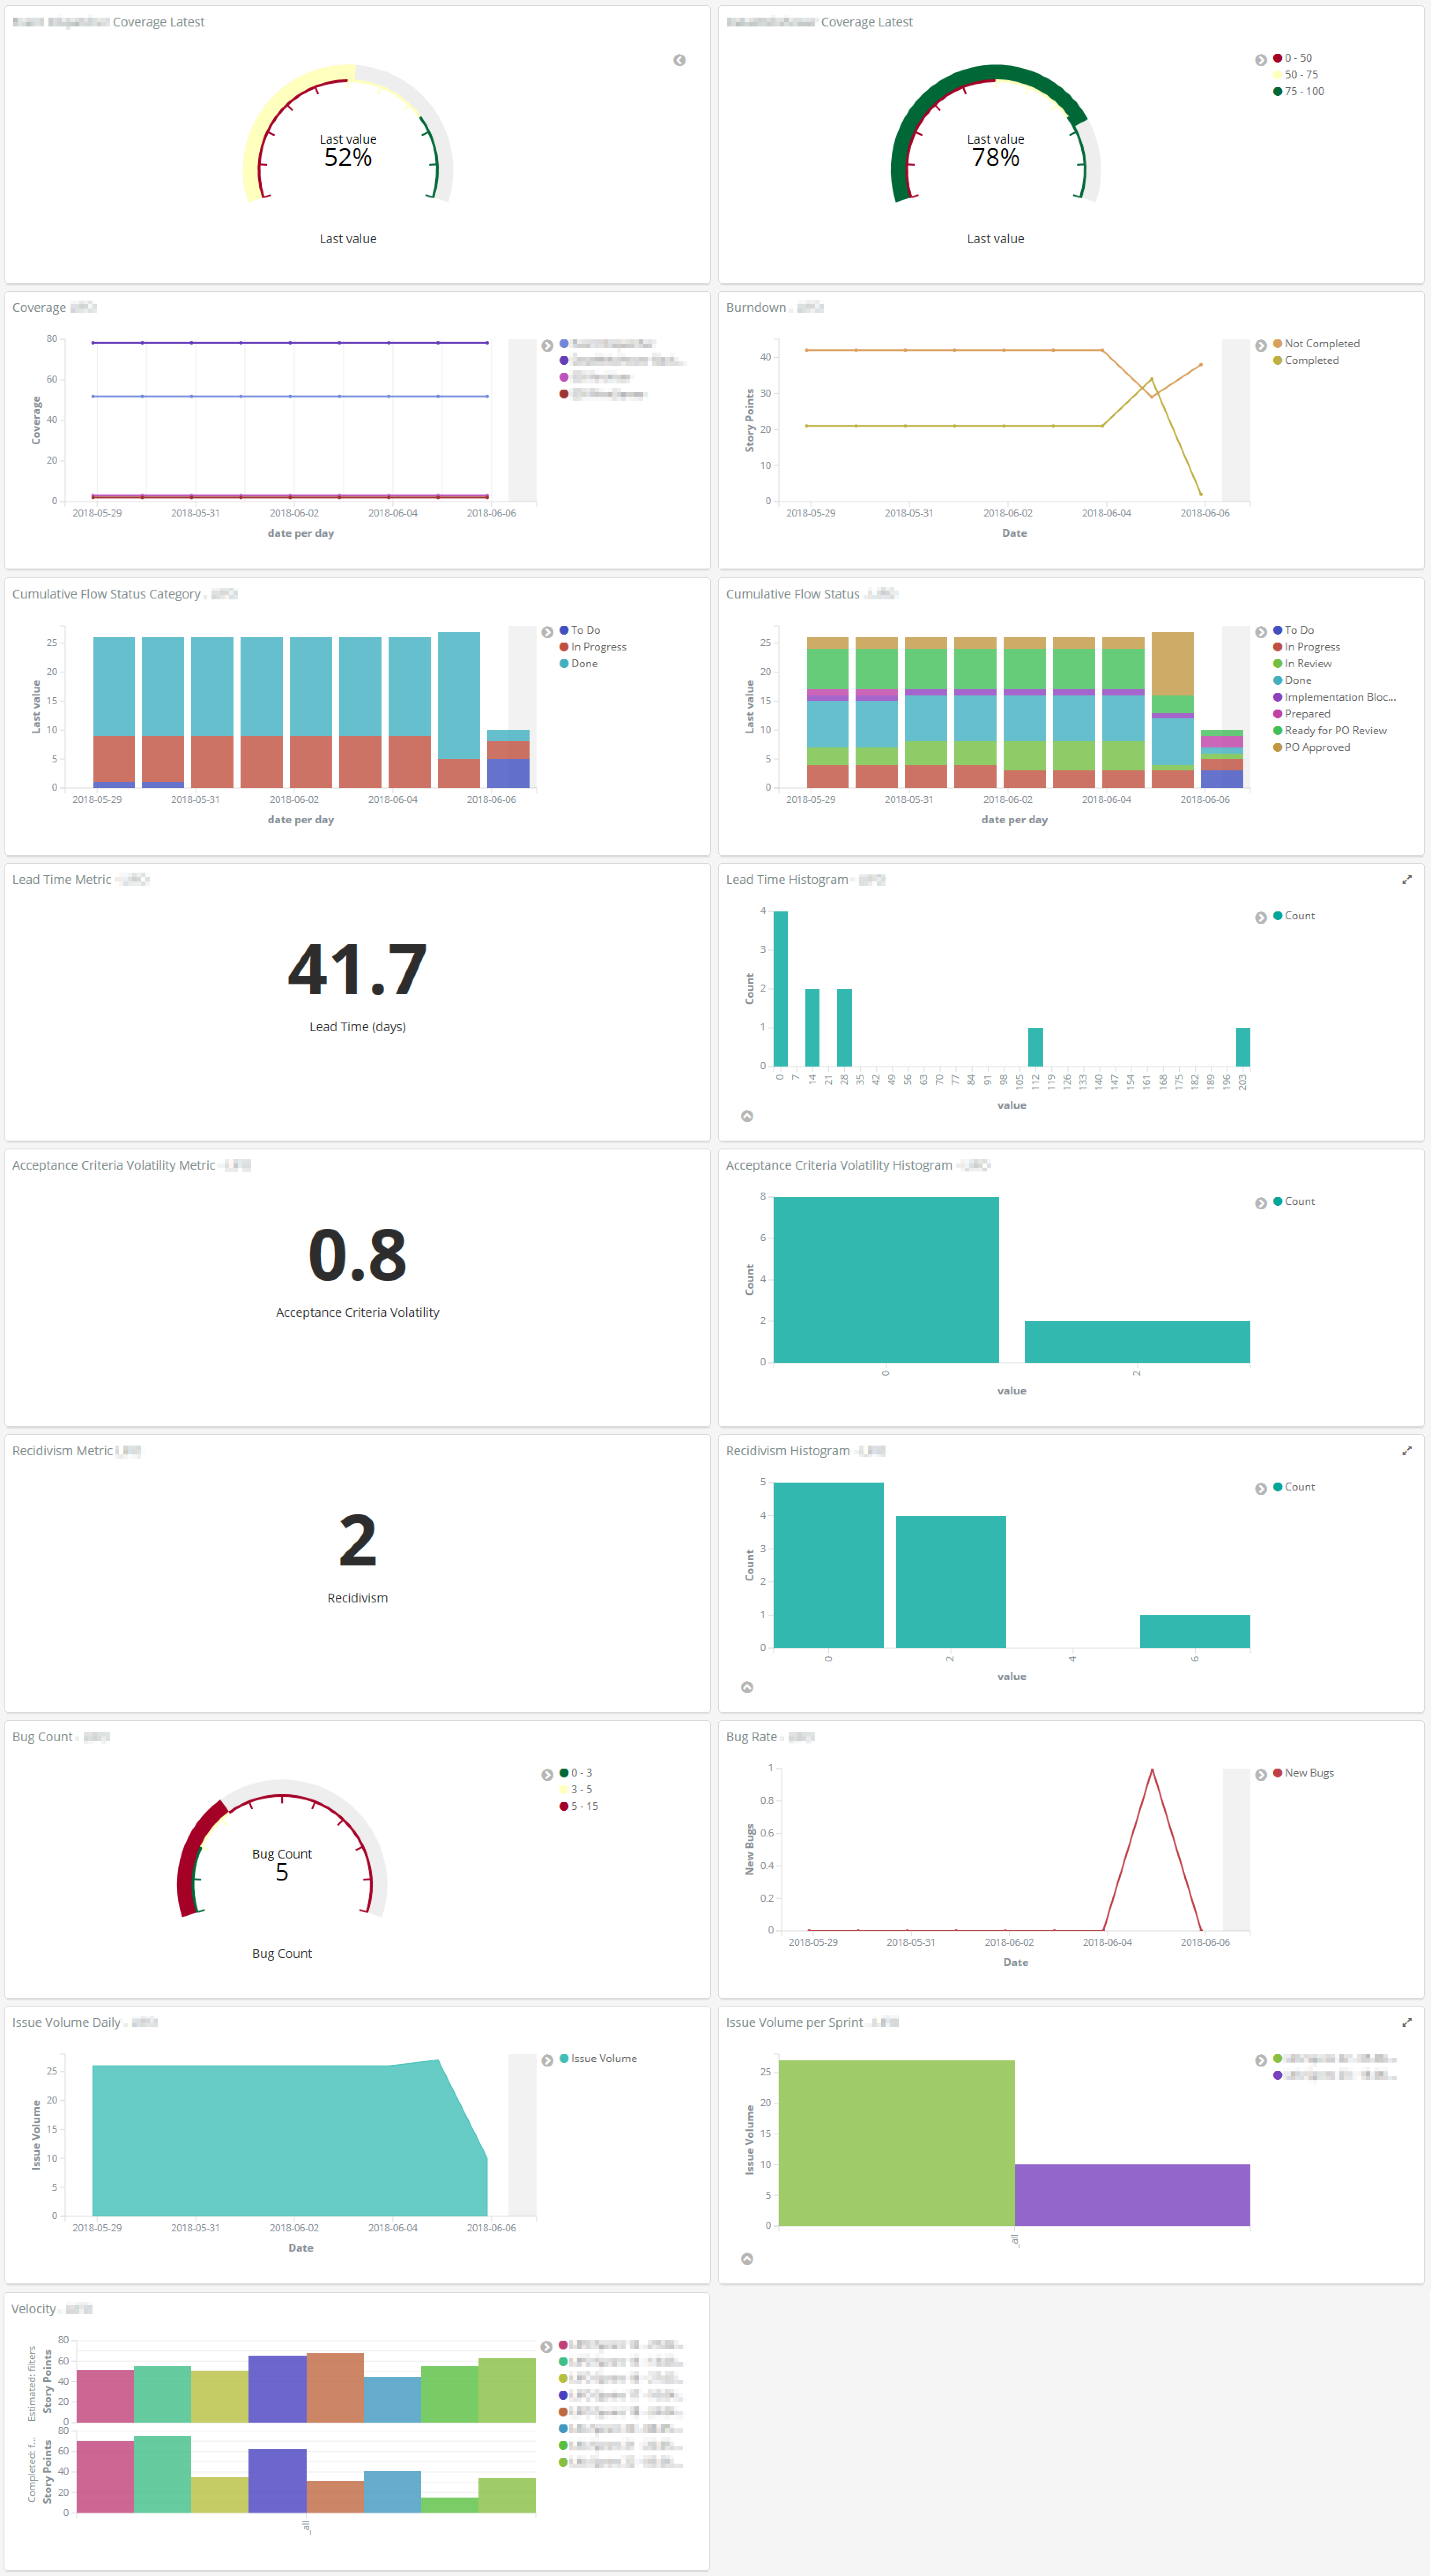
\includegraphics[width=0.7\textwidth]{img/dashboard.png}
        \caption{Dashboard mit den Metriken}\label{fig:dashboard}
    \end{figure}
\end{savenotes}

\begin{description}
    \item[Coverage] \hfill \\ Das Team hat die Verantwortung über mehrere Produkte, deshalb wurde die Testabdeckung von zwei Produkten in Form einer Messuhr dargestellt. In einem weiteren Liniendiagramm wird der Verlauf der Testabdeckung aller Produkte über die Zeit dargestellt.
    \item[Burndown] \hfill \\ Die Anzahl erledigte und noch offene Story Points im aktuellen Sprint bilden das Burndown-Chart. Es wird klassisch als Liniendiagramm dargestellt.
    \item[Cumulative Flow] \hfill \\ Beim Cumulative Flow werden nicht nur die einzelnen Statis dargestellt, sondern in einem separaten Diagramm auch noch die Status-Kategorien. Diese können bei sehr vielen unterschiedlichen Statis einen besseren Überblick bieten. Dargestellt werden beide als gestapelte Blockdiagramme, da sie einen Anteil an einem Gesamtvolumen darstellen sollen.
    \item[Lead Time] \hfill \\ Die Lead Time wird zum einen als Metrik dargestellt, zum anderen auch als Histogramm. Das hat den Grund, da hier einzelne Ausreißer nach oben oder unte die Metrik stark beeinflussen können. Das Histogramm stellt diese Ausreißer und die Verteilung noch besser dar.
    \item[Acceptance Criteria Volatility] \hfill \\ Auch bei der Flüchtigkeit der Akzeptanzkriterien wird die Metrik durch ein Histogramm ergänzt, da hier ebenfalls Ausreißer großen Einfluss haben können.
    \item[Recisivism] \hfill \\ Die Rückfälligkeit wird auch als Metrik und Histogramm dargestellt.
    \item[Bug Count und Bug Rate] \hfill \\ Die Anzahl Bugs wird als Messuhr mit bestmmten Grenzwerten dargestellt, die Bug-Rate als Liniendiagramm, um zu erkennen, wann wie viele neue Bugs erstellt wurden.
    \item[Issue Volume] \hfill \\ Das Aufgabenvolumen des aktiven Sprints wird als Flächendiagramm dargestellt. Um die Entwicklung darzustellen, wird es durch ein Blockdiagramm der Aufgabenvolumen vergangener Sprints ergänzt.
    \item[Velocity] \hfill \\ Wird als Blockdiagramm dargestellt. Sichtbar sind die geschätzen und die tatsächlich fertiggestellten Story Points pro Sprint.
\end{description}

\newpage
\subsection{Statusabfrage}

Über die RESTful Schnittstelle der Software kann der aktuelle Status abgefragt werden.

\begin{savenotes}
    \begin{figure}[H] 
        \centering
            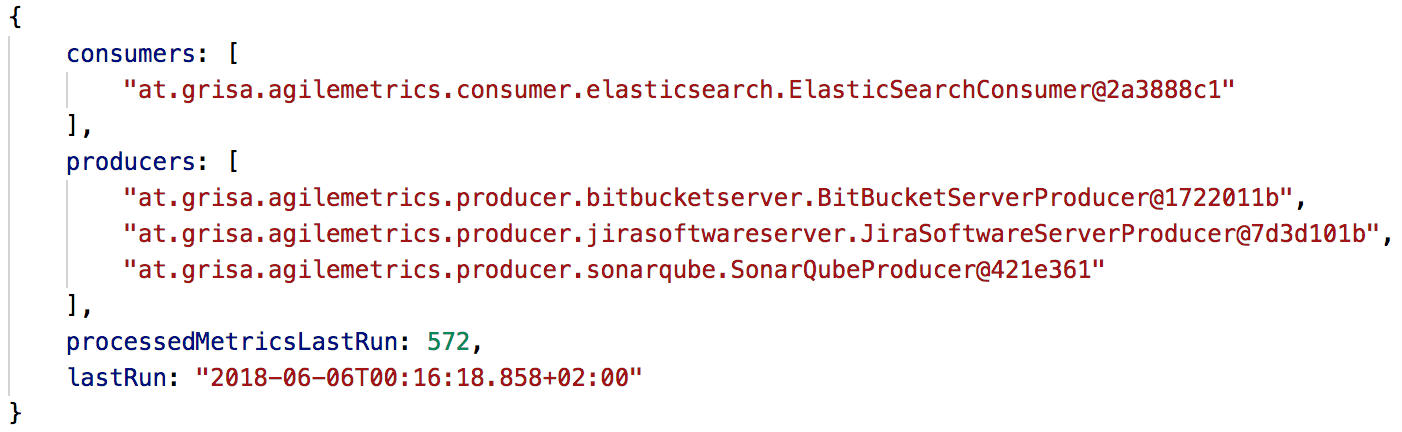
\includegraphics[width=1.0\textwidth]{img/status-api.png}
        \caption{Ergebnis der Abfrage der Statusschnittstelle}\label{fig:status-api}
    \end{figure}
\end{savenotes}

Abbildung~\ref{fig:status-api} zeigt eine solche Antwort der Schnittstelle. Ersichtlich ist eine Liste von Consumern und Producern, sowie Informationen zum letzten Lauf (Anzahl Metriken und Datum).
